\documentclass[9pt,twocolumn,twoside]{optica-suppl-materials}
\setboolean{shortarticle}{false}

\title{Cryptocurrency}

\author{Dhwani Agarwal}


\affil[1]{SY IT, Veermata Jijabai Technological Institute,Mumbai}
\affil[2]{ID NO:171081018}

\affil[*]{Corresponding author: dhwaniagarwal}

% To be edited by editor
% \dates{Compiled \today}

\begin{abstract}
Cryptocurrencies have emerged as important financial software systems. They rely on a secure distributed ledger data structure; mining is an integral part of such systems. Mining adds records of past transactions to the distributed ledger known as Blockchain, allowing users to reach secure, robust consensus for each transaction. Mining also introduces wealth in the form of new units of currency. Cryptocurrencies lack a central authority to mediate transactions because they were designed as peer-to-peer systems. They rely on miners to validate transactions. Cryptocurrencies require strong, secure mining algorithms. In this paper we survey and compare and contrast current mining techniques as used by major Cryptocurrencies. We evaluate the strengths, weaknesses, and possible threats to each mining strategy. Overall, a perspective on how Cryptocurrencies mine, where they have comparable performance and assurance, and where they have unique threats and strengths are outlined.
\end{abstract}



\begin{document}

\maketitle

\section{Introduction}

Currencies are a sort of “economic buffer”, they allow people
to convert their efforts into something that maintains its value
and can be converted back into goods or other services at a
later point in time.\\
Cryptography is the process of converting ordinary plain text
into unintelligible text and vice-versa. Modern cryptography
deals with confidentiality—information cannot be understood
by anyone, integrity—information cannot be altered, and
authentication—sender and receiver can confirm each other.\\
Putting the pieces together, Cryptocurrency is a medium of
exchange value(just like ordinary money) that exists in the
digital world and relies on encryption, which makes
transactions secure.

\section{Definitions}
Below is a list of six things that every cryptocurrency must be in
order for it to be called a cryptocurrency;
\begin{itemize}
    \item \textbf{Digital:}Cryptocurrency only exists on computers. There are no coins and no notes.
    \item \textbf{Decentralized:}Cryptocurrencies don’t have a central
computer or server. They are distributed across a network of
(typically) thousands of computers. Networks without a
central server are called decentralized networks.
     \item \textbf{Peer-to-Peer:}Cryptocurrencies are passed from person to
person online. Users don’t deal with each other through
banks, PayPal or Facebook. They deal with each other
directly. Banks, PayPal and Facebook are all trusted third
parties. There are no trusted third parties in cryptocurrency!
Note: They are called trusted third parties because users have
to trust them with their personal information in order to use
their services.
     \item \textbf{Pseudonymous:}This means that you don’t have to give any
personal information to own and use cryptocurrency. There
are no rules about who can own or use cryptocurrencies.
    \item \textbf{Trustless:}No trusted third parties means that users don’t
have to trust the system for it to work. Users are in complete
control of their money and information at all times.
    \item \textbf{Encrypted: }Each user has special codes which stop their
information from being accessed by other users. This is called
cryptography and it’s nearly impossible to hack. It’s also
where the crypto part of the crypto definition comes from.
Crypto means hidden. When information is hidden with
cryptography, it is encrypted.
    \item \textbf{Global:}Countries have their own currencies called fiat
currencies. Sending fiat currencies around the world is
difficult. Cryptocurrencies can be sent all over the world
easily. Cryptocurrencies are currencies without borders!
\end{itemize}

\section{Story Of Bitcoin}
In late 2008, Satoshi Nakamoto published the Bitcoin
whitepaper. This was a description of what Bitcoin is and how
it works. It became the model for how other cryptocurrencies
were designed in the future.\\
No one knows who Satoshi Nakamoto is. It could be a man, a
woman or even a group of people. Satoshi Nakamoto only
ever spoke on crypto forums and through emails.\\
On January 12, 2009, Satoshi Nakamoto made the first
Bitcoin transaction. They sent 10 BTC to a coder named Hal
Finney. By 2011, Satoshi Nakamoto was gone. What they left
behind was the world’s first cryptocurrency.

\section{What is Blockchain?}
\begin{condenseditemize}
    

    \item 
The thing that makes cryptocurrency different from fiat
currencies and other attempts at digital cash is blockchain
technology.
\item All cryptocurrencies use distributed ledger technology (DLT)
to remove third parties from their systems. DLTs are shared
databases where transaction information is recorded. The DLT
that most cryptocurrencies use is called blockchain technology.
\item A blockchain is a database of every transaction that has ever
happened using a particular cryptocurrency. Groups of
information called blocks are added to the database one by
one and form a very long list.
\item So, a blockchain is a linear chain of blocks! Once information
is added to the blockchain, it can’t be deleted or changed. It
stays on the blockchain forever and everyone can see it.
\item The whole database is stored on a network of thousands of
computers called nodes. New information can only be added
to the blockchain if more than half of the nodes agree that it
is valid and correct. This is called consensus. The idea of
consensus is one of the big differences between cryptocurrency
and normal banking.

\end{condenseditemize}

\section{Cryptocurrency Mining}
Cryptocurrency mining is actually more like accounting. It can be
explained with the help of Bitcoin network.\begin{condenseditemize}
    
\item For example,
George owes Michael 10 BTC. George announces that he is
sending Michael 10 BTC to the Bitcoin network.
\item Miners take the information and encrypt it. This is called
hashing. To this information, they add other transaction
information and hash that too. More and more information is
added and hashed until there is enough to form a block.
\item The miners now race against each other to guess the
encrypted code or block hash that will be given to the new
block before it’s added to the blockchain. The lucky miner
that guesses the right code gets to add the new block to the
blockchain.

\item Now, all the other nodes on the network verify the transaction
information in the new block. They check the whole
blockchain to make sure that the new information matches. If
it does, then the new block is valid, and the winning miner
can add the new block to the blockchain. This is called
confirmation.
\item Michael receives 10 BTC from George.
\end{condenseditemize}
Mining cryptocurrency uses a lot of computer power, so miners are
rewarded for the work they do. On the Bitcoin network, miners
who confirm new blocks of information are rewarded with 12.5
BTC of new Bitcoin. This is why it’s called mining. Instead of
mining for gold or coal crypto, miners are digging for new Bitcoin!\\
It’s the way cryptocurrency networks like Bitcoin verify and confirm
new transactions. It stops double spending without the need to
trust centralized accounting like banks do. Cryptocurrency
blockchains are secured by math done by computers!

\section{Figures and Tables}

\subsection{Cryptocurrency Mining}


\begin{figure}[htbp]
\centering
\fbox{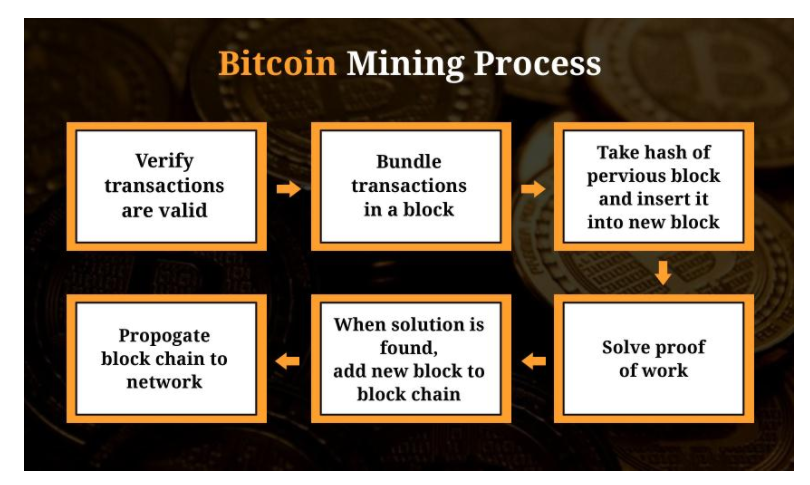
\includegraphics[width=\linewidth]{miningprocess.png}}
\caption{Mining process.}
\source{Source:https://www.webopedia.com/TERM/C/cryptocurrency-mining.html}
\label{fig:false-color}
\end{figure}

\subsection{Blockchain}


\begin{figure}[htbp]
\centering
\fbox{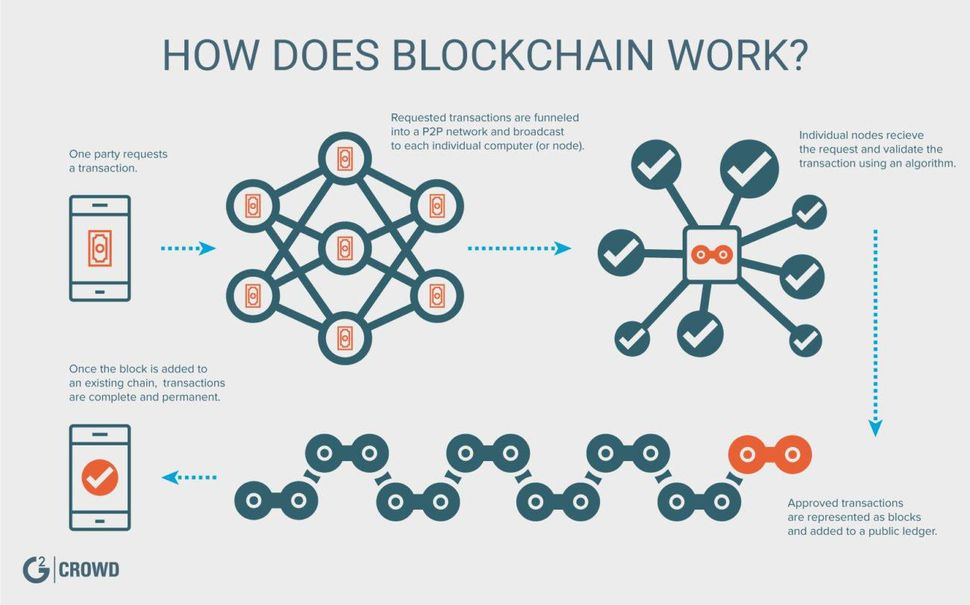
\includegraphics[width=\linewidth]{blockchain-graphic-g2.jpg}}
\caption{Working of Blockchain.}
\source{Source: https://blockgeeks.com/guides/what-is-blockchain-technology/}
\label{fig:false-color}
\end{figure}



\subsection{Traditional currency VS Cryptocurrency}
The below table gives us the exact difference between real worlsd currency and cryptocurrency on the basis of different aspects:
\\
\bigskip
\bigskip
\bigskip
\bigskip
\bigskip


\begin{table}[htbp]
\centering
\caption{\bf Comparison}
\begin{tabular}{|p{2cm}|p{3cm}|p{3cm}|}
\hline
Points of comparison & Tradition currency & Cryptocurrency\\
\hline
Authority & Executives responsible to shareholders and directors & Decentralized\\
\hline
Trust & You have to trust the financial immediatry who handles the money & You have to trust the code \\
\hline
Data & Segmented in organized chunks placed in central servers under the control of one legal entity & Distributed in chains of blocks,placed in servers around the world.  \\
\hline
\end{tabular}
  \label{tab:shape-functions}
\end{table}

\section{Conclusion}
Summing up, cryptocurrency is a radically new way of paying
that makes all the transactions secure and helps to get rid of
intermediaries represented by banks, which also contributes to
a significant reduction in the commission fee.\\
The main feature of cryptocurrencies—security which is
provided by Blockchain technology—a network of computers
having an identical copy of the database and changing its
records by a common agreement based on pure mathematics.

\begin{thebibliography}{}
\bibitem{}https://www.bitdegree.org/tutorials/what-is-cryptocurrency
\bibitem{}https://medium.com/
\bibitem{}Wikipedia

\end{thebibliography}

% Bibliography


%Manual citation list
%\begin{thebibliography}{1}
%\bibitem{Zhang:14}
%Y.~Zhang, S.~Qiao, L.~Sun, Q.~W. Shi, W.~Huang, %L.~Li, and Z.~Yang,
 % \enquote{Photoinduced active terahertz metamaterials with nanostructured
  %vanadium dioxide film deposited by sol-gel method,} Opt. Express \textbf{22},
  %11070--11078 (2014).
%\end{thebibliography}

\end{document}